\documentclass[cn]{elegantbook}
\usepackage[square,numbers,sort&compress]{natbib}
\newcommand{\upcite}[1]{\textsuperscript{\textsuperscript{\cite{#1}}}}
\usepackage{diagbox}
\usepackage{algorithm}
\usepackage{algorithmicx}
\usepackage{algpseudocode}
\renewcommand{\algorithmicrequire}{\textbf{输入:}}
\renewcommand{\algorithmicensure}{\textbf{输出:}}

\tikzstyle{startstop} = [rectangle, rounded corners, minimum width = 2cm, minimum height=1cm,text centered, draw = black, fill = red!40]
\tikzstyle{arrow} = [->,>=stealth]

% title info
\title{模式识别作业3}
\subtitle{分类问题}
% bio info
\author{罗雁天}
\institute{清华大学电子系}
\version{2018310742}
\date{\today}
\logo{logo.png}
\cover{cover.jpg}

\begin{document}

\maketitle
\tableofcontents
\mainmatter
\hypersetup{pageanchor=true}
% add preface chapter here if needed
\chapter{线性分类问题}
\section{问题描述}
\noindent 给定两组数据:
\begin{equation}
\begin{aligned}
\omega_1&=\{(2,3); (2,2); (2,4); (3,3); (3,4); (2.5,3); (1.5,2); (3.5,2.5); (4,4); (0.5,0.5)\} \\
\omega_2&=\{(0,2.5); (-2,2); (-1,-1); (1,-2); (3,0); (-2,-2); (-3,-4); (-5,-2); (4,-1)\}
\end{aligned}
\end{equation}
求出其识别函数、识别界面以及绘制出识别界面将该训练样本的区分结果。

\section{最小欧式距离分类}
\subsection{算法描述}
\noindent 使用最小欧式距离对此问题进行二分类,我们有如下算法Algorithm \ref{alg:mindis}
\begin{algorithm}[htb]
	\caption{最小欧式距离二分类}
	\label{alg:mindis}
	\begin{algorithmic}[1]
		\Require $\omega_1, \omega_2$
		\Ensure 识别函数,分类界面
		\State 计算两个类的类中心:$M_i=\frac{1}{N_i}\sum_{X\in \omega_i}X,\quad i=1,2$
		\State 计算$d_i(x)=x^T\cdot M_i-\frac{1}{2}M_i^T\cdot M_i,\quad i=1,2$
		\State 所以识别函数为:$f(x)=\left\{\begin{array}{cc}
		x\in class1 & \mbox{如果}d_1\ge d_2 \\
		x\in class2 & \mbox{如果}d_1<d_2
		\end{array}\right.$
		\State 设分类界面上任意一点为$p=(p_1,p_2)^T$
		\State 则分类界面为:$\left(p^T-\frac{M_1^T+M_2^T}{2}\right)\cdot (M_1-M_2)=0$
	\end{algorithmic}
\end{algorithm}

\subsection{实验结果}
使用Algorithm \ref{alg:mindis},我们计算出:
\begin{equation}
\begin{aligned}
M_1&=[2.4,2.8]^T \\
M_2&=[-0.5556,-0.8333]^T
\end{aligned}
\end{equation}

那么对于任意的数据点$\mathbf{x}=[x_1,x_2]^T$,我们有:
\begin{equation}
\begin{aligned}
d_1&=x^T\cdot M_1-\frac{1}{2}M_1^T\cdot M_1=2.4x_1+2.8x_2-6.8 \\
d_2&=x^T\cdot M_2-\frac{1}{2}M_2^T\cdot M_2=-\frac{5}{9}x_1-\frac{5}{6}x_2-\frac{325}{648}
\end{aligned}
\end{equation}

所以我们的识别函数为:
\begin{equation}
f(\mathbf{x})=\left\{
\begin{array}{cc}
x\in class1 & \mbox{如果}d_1\ge d_2 \\
x\in class2 & \mbox{如果}d_1<d_2
\end{array}
\right.
\end{equation}

设分类界面上任意一点为$p=(p_1,p_2)^T$,那么我们可以得到分类界面为:
\begin{equation}
\begin{aligned}
&\left(p^T-\frac{M_1^T+M_2^T}{2}\right)\cdot (M_1-M_2)=0 \\
\Rightarrow&2.9556p_1+3.6333p_2-6.2985=0
\end{aligned}
\end{equation}

绘制出分类界面如图\ref{res1}所示
\begin{figure}[!h]
	\centering
	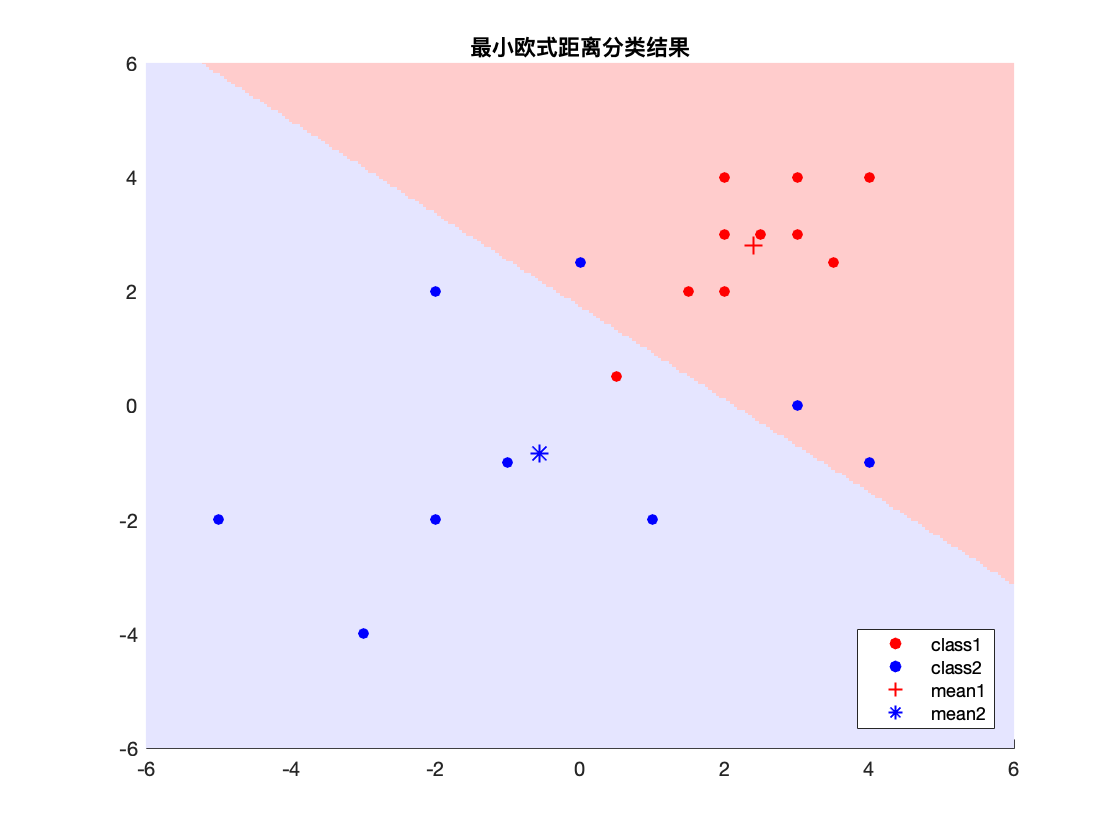
\includegraphics[width=\textwidth]{../results/LD}
	\caption{\label{res1}使用最小欧式距离分类所得的分类界面示意图}
\end{figure}

我们可以统计出class1和class2的召回率和虚警率如表\ref{tab1}所示,从中可以看出,最小距离分类会带来一定的虚警率,class2误判为class1的较多。
\begin{table}[!h]
	\centering\caption{\label{tab1}最小欧式距离分类的召回率和虚警率}
	\begin{tabular}{|c|c|c|}
		\hline
		类别 & 召回率 & 虚警率 \\
		\hline
		class1 & 9/10 & 3/9 \\
		\hline
		class2 & 6/9 & 1/10 \\
		\hline
		\end{tabular}
\end{table}

\section{支持向量机SVM分类}
\subsection{算法描述}
SVM的目标是寻找一个超平面,使得它不仅能正确地分类每一个样本,并且要使得每一类样本中距离超平面最近的样本到超平面的距离尽可能远。可以将其转换为求解如下优化问题:
\begin{equation}
\begin{aligned}
\min \quad&\frac{1}{2}w^Tw\\
s.t.\quad&y_i(w^Tx_i+b)\ge 1
\end{aligned}
\end{equation}
其中,$(x_i,y_i)$是训练样本,$y_i\in\{1,-1\}$,$w,b$为超平面的权重。对于此优化问题,我们可以使用拉格朗日对偶转换为对偶问题,对偶问题可以化简为:
\begin{equation}
\begin{aligned}
\min \quad&-\frac{1}{2}\sum_{i=1}^{l}\sum_{j=1}^l\alpha_i\alpha_jy_iy_jx_i^Tx_j+\sum_{i=1}^l\alpha_i\\
s.t.\quad&\alpha_i\ge 0,\quad i=1,2,\cdots,1\\
&\sum_{i=1}^l\alpha_iy_i=0
\end{aligned}
\end{equation}
然后求解此二次规划问题便可以得到分类界面。
\subsection{实验结果}
使用SVM分类的结果如图\ref{res4}所示:
\begin{figure}[!ht]
	\centering
	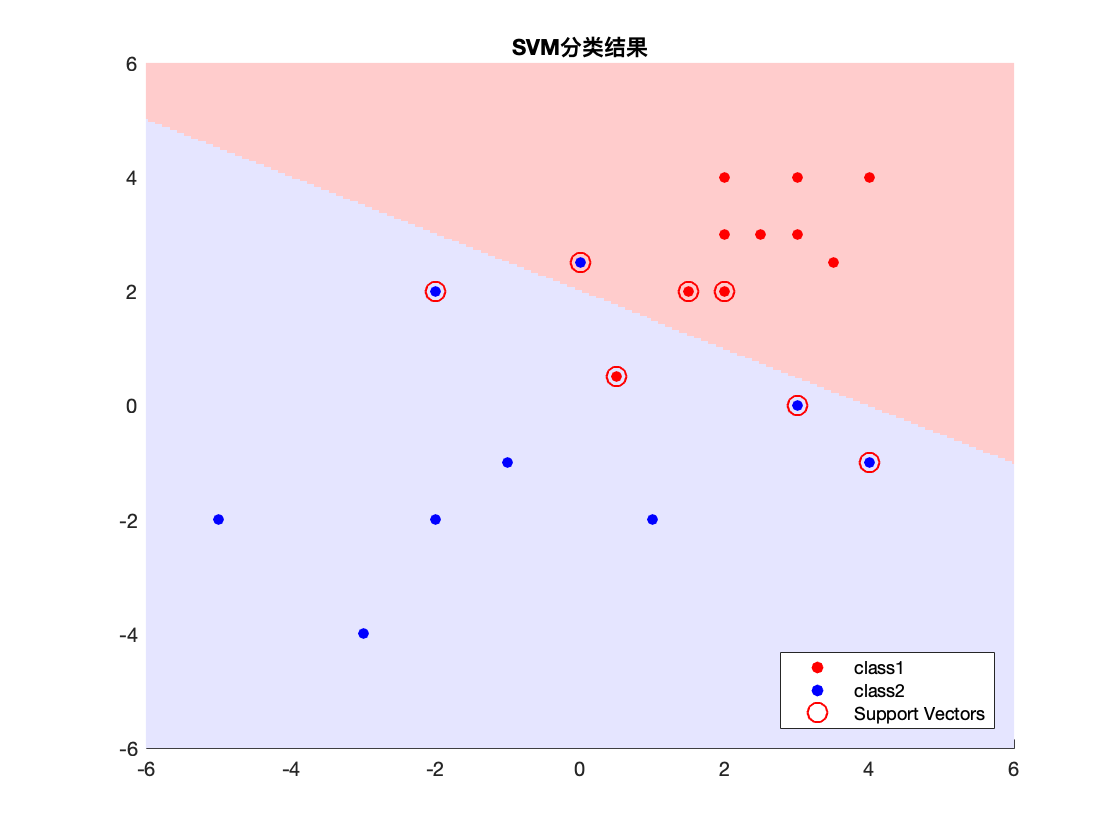
\includegraphics[width=\textwidth]{../results/LD2}
	\caption{\label{res4}使用最小欧式距离分类所得的分类界面示意图}
\end{figure}

同样,我们也统计出此种方法下class1和class2的召回率和虚警率如表\ref{tab2}所示,从中可以看出,使用SVM分类的效果要比最小欧式距离分类的效果好。

\begin{table}[!h]
	\centering\caption{\label{tab2}SVM分类的召回率和虚警率}
	\begin{tabular}{|c|c|c|}
		\hline
		类别 & 召回率 & 虚警率 \\
		\hline
		class1 & 9/10 & 1/9 \\
		\hline
		class2 & 8/9 & 1/10 \\
		\hline
	\end{tabular}
\end{table}
\chapter{非线性分类问题}
\section{问题描述}
如图\ref{ex2}所示,求分离{\color{red}$\bullet$}和
\begin{tikzpicture}
\fill[green!60!black] (0,0) -- (0.22,0.39) -- (0.44,0) -- cycle;
\end{tikzpicture}的函数


\begin{figure}[!h]
	\centering
	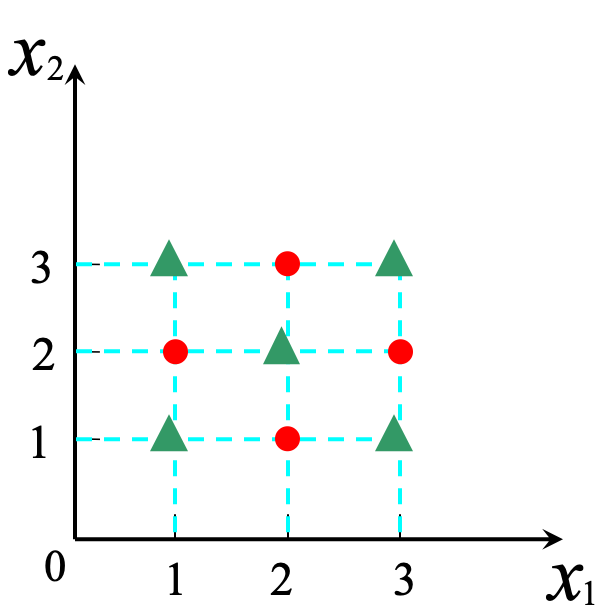
\includegraphics[width=0.4\textwidth]{images/ex2}
	\caption{\label{ex2}非线性分类问题}
\end{figure}

\section{非线性映射法}
在本小节,我们首先使用非线性映射,将二维数据升到三维,然后再使用Algorithm \ref{alg:mindis}中提到的最小欧式距离分类算法进行分类。

\subsection{算法设计}
观察数据点的分布可以看出,正负样本可以通过两个等轴双曲线进行分类,因此,对任意的数据点$\mathbf{x}=[x_1,x_2]^T$我们首先设计了如下的非线性映射函数:
\begin{equation}
\phi_1(x_1,x_2)=\left[x_1,x_2,\left((x_1-2)^2-(x_2-2)^2\right)^2\right]
\end{equation}

在经过非线性映射之后,我们便可以将其看做是三维空间的线性分类问题,使用算法Algorithm \ref{alg:mindis}或者线性SVM便可求出分类界面。

从数据点的分布我们还可以看出,可以通过两个同心圆对数据进行分类,因此我们设计了如下的非线性映射函数:
\begin{equation}
\phi_2(x_1,x_2)=\left[x_1, x_2, \left((x_1-2)^2+(y_1-2)^2-1\right)^2\right]
\end{equation}

同样,转换之后可以用线性分类的方法进行分类。

\subsection{实验结果}
\subsubsection{线性最小欧氏距离+非线性映射实验结果}
使用上一小节设计的两种非线性映射函数进行线性最小欧氏距离分类实验,可以得到如图\ref{res2}和\ref{res3}所示的分类界面,可以看出分类结果正确,使用非线性映射的方式成功将线性不可分的问题转化为线性可分问题。

\begin{figure}[!h]
	\centering
	\begin{minipage}{0.48\linewidth}
		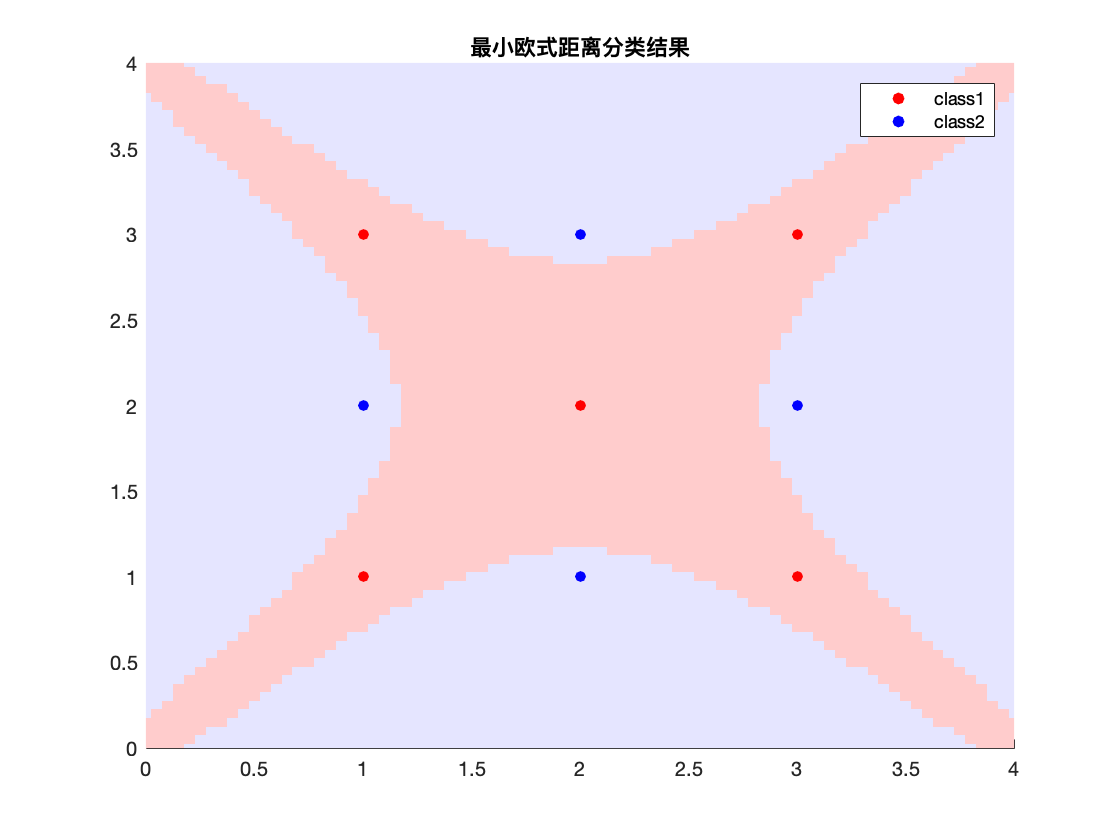
\includegraphics[width=\textwidth]{../results/non1}
		\caption{\label{res2}最小欧式距离分类+非线性映射1的分类界面示意图}
	\end{minipage}
	\begin{minipage}{0.48\linewidth}
		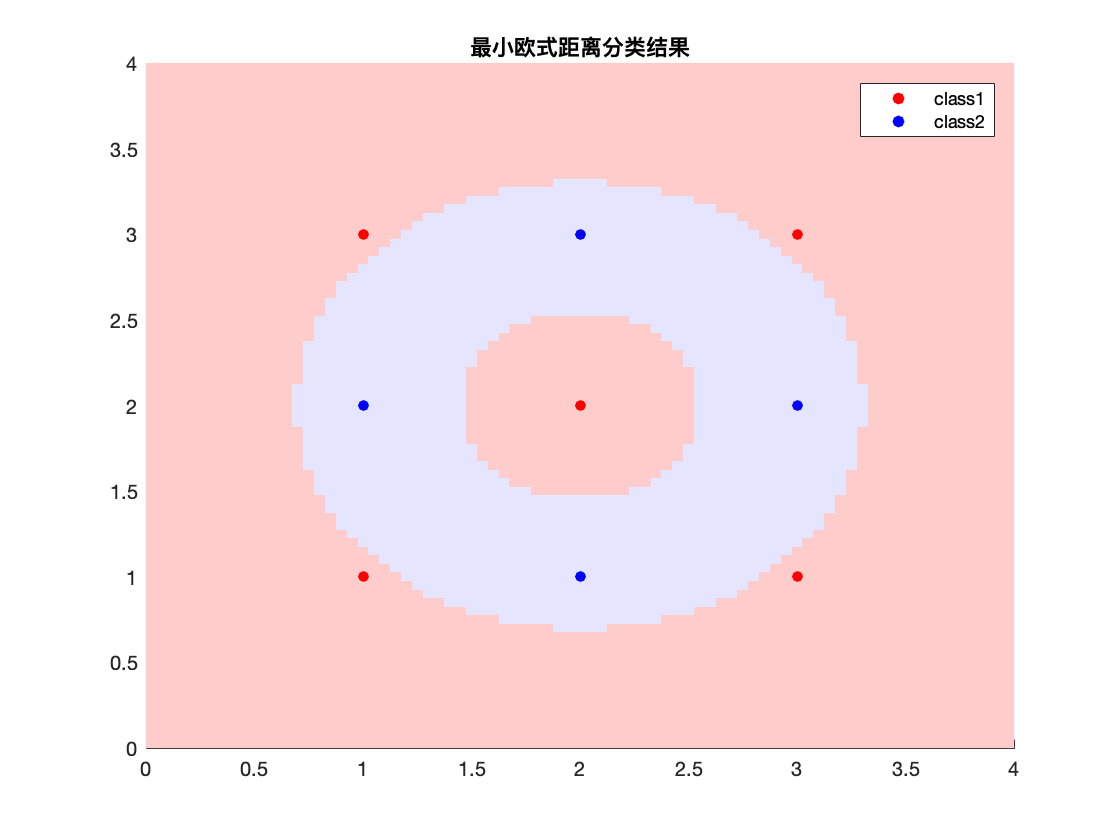
\includegraphics[width=\textwidth]{../results/non2}
		\caption{\label{res3}最小欧式距离分类+非线性映射2的分类界面示意图}
	\end{minipage}
\end{figure}

\subsubsection{SVM+非线性映射实验结果}
使用上一小节设计的两种非线性映射函数进行线性SVM分类实验,可以得到如图\ref{res5}和\ref{res6}所示的分类界面,可以看出分类结果正确,使用非线性映射的方式成功将线性不可分的问题转化为线性可分问题。

\begin{figure}[!h]
	\centering
	\begin{minipage}{0.48\linewidth}
		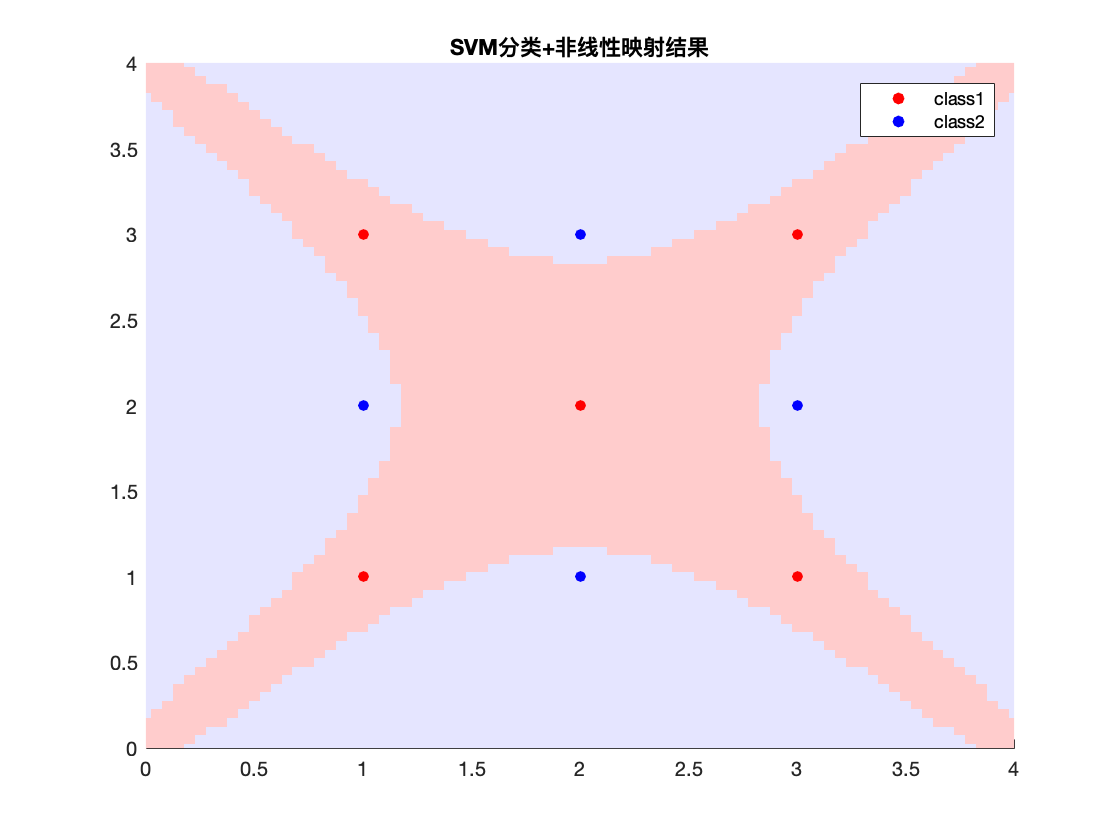
\includegraphics[width=\textwidth]{../results/non3}
		\caption{\label{res5}SVM分类+非线性映射1的分类界面示意图}
	\end{minipage}
	\begin{minipage}{0.48\linewidth}
		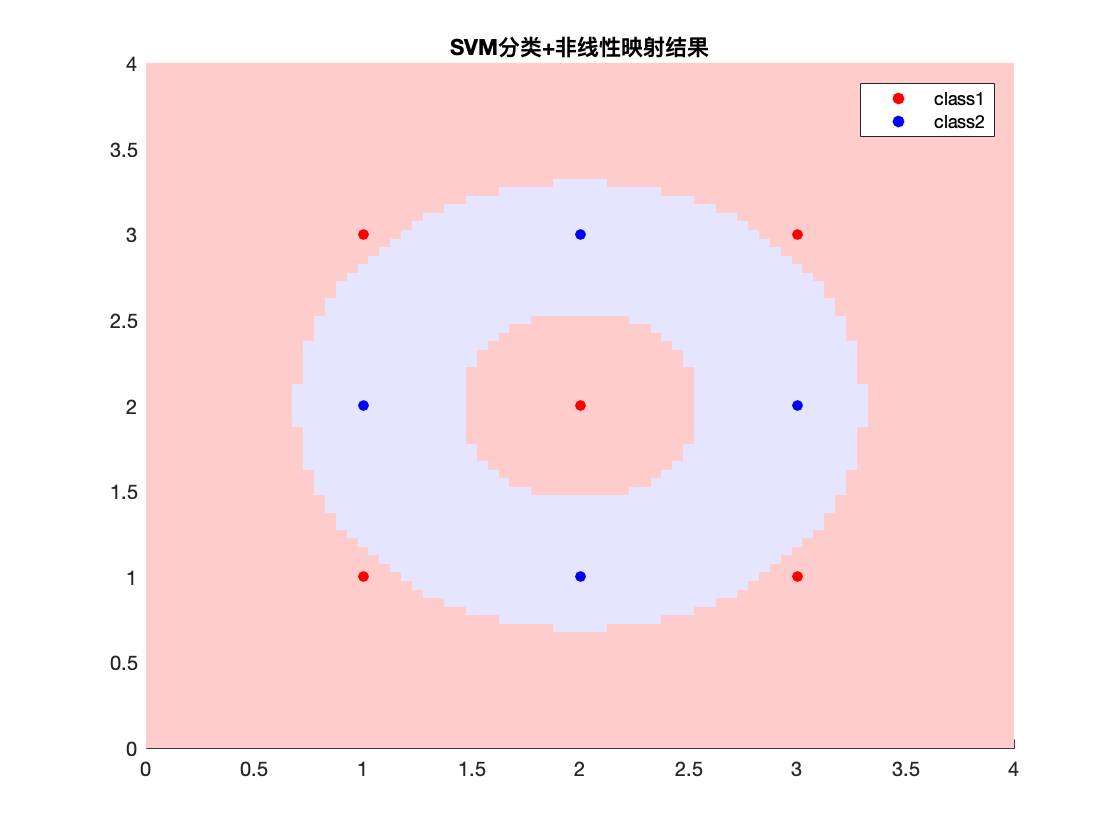
\includegraphics[width=\textwidth]{../results/non4}
		\caption{\label{res6}SVM分类+非线性映射2的分类界面示意图}
	\end{minipage}
\end{figure}

\section{SVM+核函数方法}
在使用SVM中,我们可以使用核函数来代替非线性映射的方式对非线性问题进行分类,具体而言,构造核函数$k(x_1,x_2)$使得:
\begin{equation}
k(x_1,x_2)=\phi(x_1)^T\phi(x_2)
\end{equation}
这样便可以将线性SVM中最后的优化问题转换为:
\begin{equation}
\begin{aligned}
\min \quad&-\frac{1}{2}\sum_{i=1}^{l}\sum_{j=1}^l\alpha_i\alpha_jy_iy_jk(x_i,x_j)+\sum_{i=1}^l\alpha_i\\
s.t.\quad&\alpha_i\ge 0,\quad i=1,2,\cdots,1\\
&\sum_{i=1}^l\alpha_iy_i=0
\end{aligned}
\end{equation}
常见的核函数有RBF、Gaussian、polynomial等核函数,在此我们选择polynomial核函数进行实验,绘制出分类界面如图\ref{res7}所示,可以看出并没有完全分类正确,因此,使用polynomial核函数的SVM相比于自己设计非线性映射的效果更差一些。
\begin{figure}[!h]
	\centering
	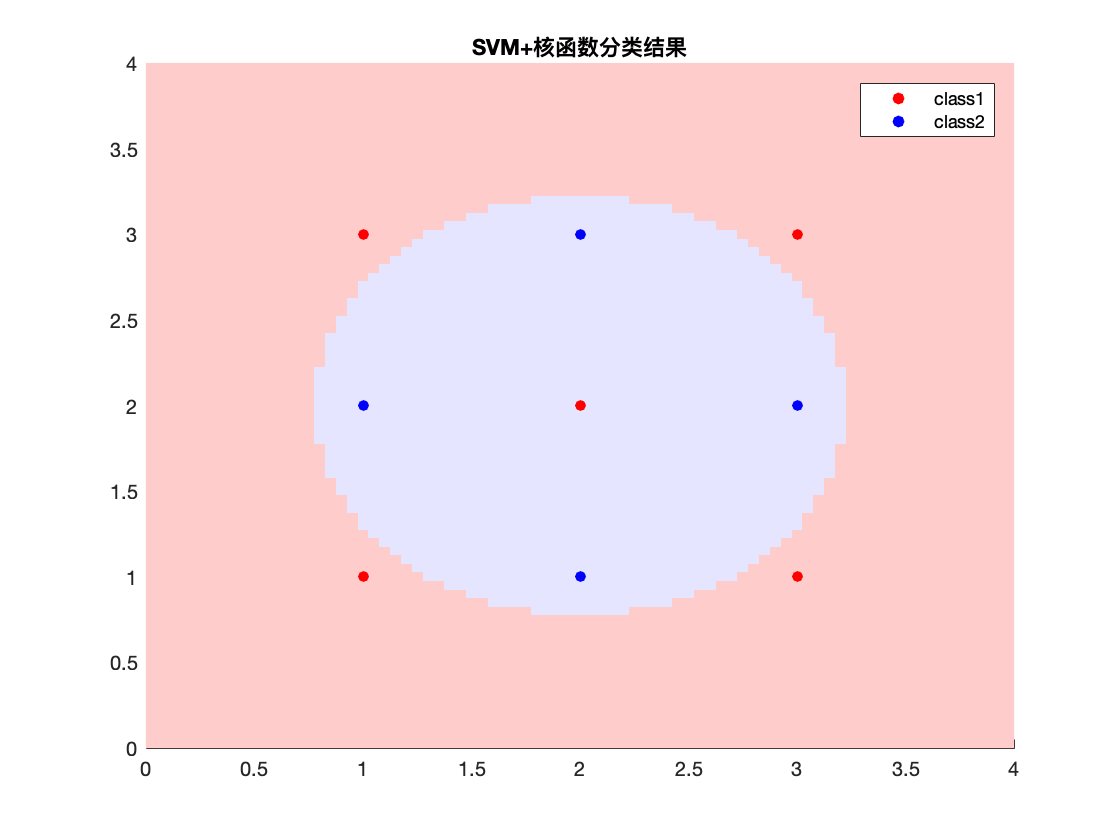
\includegraphics[width=0.7\textwidth]{../results/non5}
	\caption{\label{res7}SVM分类+核函数的分类界面示意图}
\end{figure}

\section{总结}
从提出的三种非线性分类的算法来看,设计好的非线性映射能够带来好的分类效果,使用最小欧式距离分类+非线性映射算法和SVM分类+非线性映射算法分类效果较好,而使用polynomial核函数的分类效果就比较差了。因此,对于不同的非线性分类问题,设计一种较好的非线性映射是一个较好的方法,但是需要针对不同问题分别设计,这样鲁棒性不高。
\chapter{代码说明}
\noindent 本次实验使用Matlab语言编写,所有代码放置在“code/”文件夹下:
\begin{itemize}
	\item linearclassify.m: 线性分类的主程序,直接执行便可以得到分类界面;
	\item plot\_boundary.m: 绘制线性分类器的分类界面;
	\item nonlinearclassify.m: 非线性分类的主程序,直接执行便可以得到分类界面;
	\item mykernel.m: 设计的非线性映射函数。
\end{itemize}


\end{document}